\documentclass[10pt, compress]{beamer}

\usetheme{m}

\usepackage{booktabs}
\usepackage[scale=2]{ccicons}
\usepackage{minted}
\usepackage{tikz}
\usetikzlibrary{calc, arrows}
\usepackage{xstring}
\usepackage{amsmath}
\usepgfplotslibrary{dateplot}
\usemintedstyle{trac}


\usetikzlibrary{shapes,arrows}
\tikzstyle{cloud} = [draw, ellipse, node distance=4cm,    minimum height=2em]
\tikzstyle{cloudgreen} = [draw, ellipse, fill=green!20, node distance=4cm,    minimum height=2em]
\tikzstyle{blockred} = [rectangle, draw, fill=red!20, 
text width=5em, text centered, rounded corners, minimum height=4em, minimum width= 6em]
\tikzstyle{block} = [rectangle, draw, fill=white!20, 
text width=5em, text centered, rounded corners, minimum height=4em,minimum width= 6em]
\tikzstyle{blockgreen} = [rectangle, draw, fill=green!20, 
text width=5em, text centered, rounded corners, minimum height=4em, minimum width= 6em]
\tikzstyle{line} = [draw, -latex']


\renewcommand{\(}{\begin{columns}}
\renewcommand{\)}{\end{columns}}
\newcommand{\<}[1]{\begin{column}{#1}}
	\renewcommand{\>}{\end{column}}
%%%%%%%%%%%%%%%%%%%%%%%%%%%%%%%%%%%%%%%%%%%%%%%%%%
\newcommand*{\NodeSize}{0.5cm}%
\newcommand*{\YShiftBetweenRows}{-1cm}% Subsequent rows are shited down so they don't overlap
\tikzset{DNA Style/.style={minimum size=0.5cm, draw=gray, line width=1pt}}{}

\newlength{\YShift}% 
\newcounter{ColumnCounter}% Prefix for node labels

% Initialize - These are probably not needed, but prefer to set them
\setlength{\YShift}{0cm}% 
\setcounter{ColumnCounter}{0}
\newcommand*{\DNASequence}[2][Mark]{%
	% http://tex.stackexchange.com/questions/12091/tikz-foreach-loop-with-macro-defined-list
	\def\Sequence{#2}
	\foreach [count=\xi] \Label/\Color in \Sequence {%
		\pgfmathsetmacro{\XShift}{\NodeSize*\xi}%
		\IfStrEq{\Color}{}{\def\Color{white}}{}
		\edef\NodeName{#1-\arabic{ColumnCounter}}
		\node [DNA Style, fill=\Color, xshift=\XShift] (\NodeName) {\Label};
		\stepcounter{ColumnCounter}
	} 
}%
\newcommand*{\ThreeDNASequences}[4][Mark]{% #1 = tikzmark prefix
	\setcounter{ColumnCounter}{0}% reset column counter
	\begin{scope}[yshift=\YShift]
		\DNASequence[#1]{#2} 
		\pgfmathsetmacro{\Shift}{6cm}% Should compute this based on num of items in #1
		\begin{scope}[xshift=\Shift]
			\DNASequence[#1]{#3} 
		\end{scope}
		\pgfmathsetmacro{\Shift}{8cm}% Should compute this based on num of items in #2  
		\begin{scope}[xshift=\Shift]
			\DNASequence[#1]{#4} 
		\end{scope}
	\end{scope}
	\pgfmathsetlength{\YShift}{\YShift\YShiftBetweenRows}%
}

\title{Computational analysis of cell-to-cell heterogeneity in single-cell RNA-sequencing data reveals hidden subpopulations of cells}
\subtitle{Buettner et al., (2015) Nature Biotechnology, 1–32. doi:10.1038/nbt.3102}

\vspace*{20pt}
\author[skc]{Saket Choudhary}
%\institute{\inst{1} University of Southern California}

\date{%\vspace*{50pt}
\today \\
BISC 542}

\begin{document}

\maketitle


\begin{frame}[fragile]
\frametitle{Outline}
\begin{itemize}
\item Motivation
\item Methods[Overview]
\item Results
\item Challenges \& Possibilities
\item Conclusion
\end{itemize}
\end{frame}

\section{Motivation}
\begin{frame}[fragile]
\frametitle{Single Cell sequencing: Challenges}
\begin{itemize}[<+- | alert@+>]
\item Limited amount of sample: Prone to noise and contamination
\item Profiling hundreds of cells: How to identify subpopulations?
\item Identify regulatory landscape of each cell population
\item \textbf{Account for hidden confounding factors that might explain cell heterogeneity}
\end{itemize}
\end{frame}

\begin{frame}[fragile]
\frametitle{What was it all about?}
\begin{itemize}
\item Single cell transcriptomics heterogeneity: many single cells at the same time
\item Accounting for technical noise was a solved problem; how do you account for \textit{other} sources of variability: cell cycle,
differentiation state etc.
\item Given expression levels, how do you infer the effect of \textit{latent} variables
\end{itemize}
Key focus: How does cell cycle affect expression levels?
Given the apriori nature of genes(association with cell-cycle), is it possible to remove the effect of cell cycles?

\end{frame}


\begin{frame}[fragile]
\frametitle{What was it all about?}
\frametitle{Goals}
\begin{itemize}[<+- | alert@+>]
\item Separate out different sources of variation : \textit{technical}, \textit{biological}, \textit{cell cycle}, \textit{other hidden factors}
with the idea of studying the underlying \textit{interesting} biology. \\

\item Variations such as cell cycle can mask out more physiologically important differences.\\

\item Focusing on cells that have \textit{paused} such as terminally differentiated nuerons will give a limited view

\item Measuring in bulk would have simply given a weighted observable

\item Decomposition of this variance by splitting it for different confounding factors can really useful.
If the original interest is in studying effect of differentiation, it makes sense to factor out the
effect of cell cycle. \\


\item Discovering previously unidentified cell types?! \\
\end{itemize}
\end{frame}


\section{Methods}
\begin{frame}[fragile]
\frametitle{Method in a gist}
\begin{itemize}[<+- | alert@+>]
\item Two step approach: Reconstruct state of unobserved factors; Use this information to perform correction over gene 
expression values
\item Learn from a pool of well annotated gene sets, those related to cell cycle
\item Uses bayesian technique to infer effect of latent variables
\item Fit a \textit{low-rank} covariance matrix to a set of \textbf{predefined} marker genes
\item Estimate the state of hidden factors using maximum likelihood approach
\item Decompose the variability of expression levels \textit{across} single cells: expression = mean effect + random effect
\item Regress out effects of hidden factors
\item Corrected gene expression level

\end{itemize}
Details later...
\end{frame}

\section{Results}
scLVM: single Cell Latent variable Models
\begin{frame}
\frametitle{Cell cycle affects global gene expression}
\begin{figure}
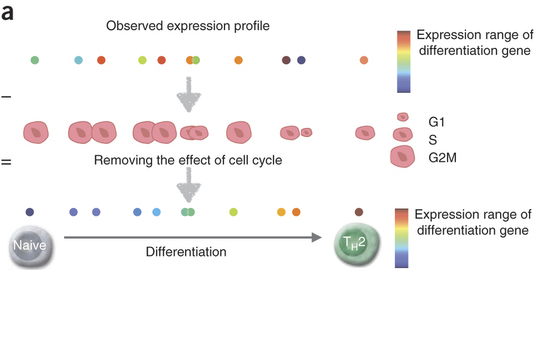
\includegraphics[width=0.8\linewidth]{images/expression.jpg}
\caption{Observed Expression = Effect of differentiation + Effect of state of cell($G1,  S , G2$)}
\end{figure}
\end{frame}

\begin{frame}
\frametitle{Cell cycle affects can be controlled by fitting a cell-cell covariance matrix}
\begin{figure}
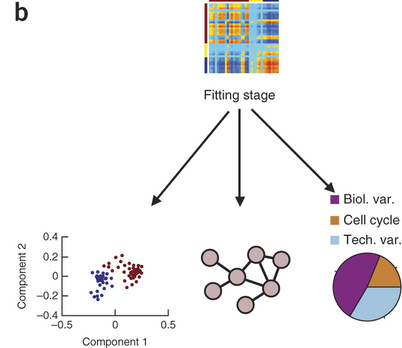
\includegraphics[width=0.5\linewidth]{images/fitting.jpg}
\caption{Inferring the cell-cell covariance matrix using hidden factors such as the cell cycle. This is then used to calculate adjusted
gene expression values for downstream analysis}
\end{figure}
\end{frame}



\begin{frame}
\frametitle{Validation}
\begin{figure}
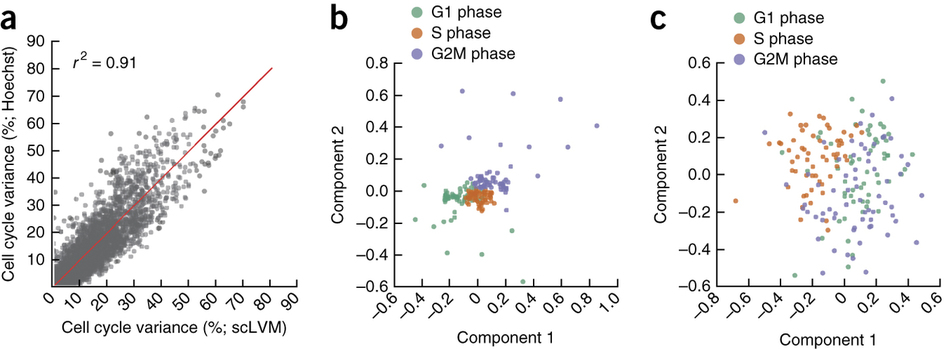
\includegraphics[width=0.8\linewidth]{images/results1.jpg}
\caption{a. Gold standard v/s scLVM agreement
b.Non Linear PCA on scLVM corrected data: no separation c.nonlinear PCA on unorrected data: separation by cell cycle!}
\end{figure}
\end{frame}

%\begin{frame}
%\frametitle{Results in a gist}
%\begin{figure}
%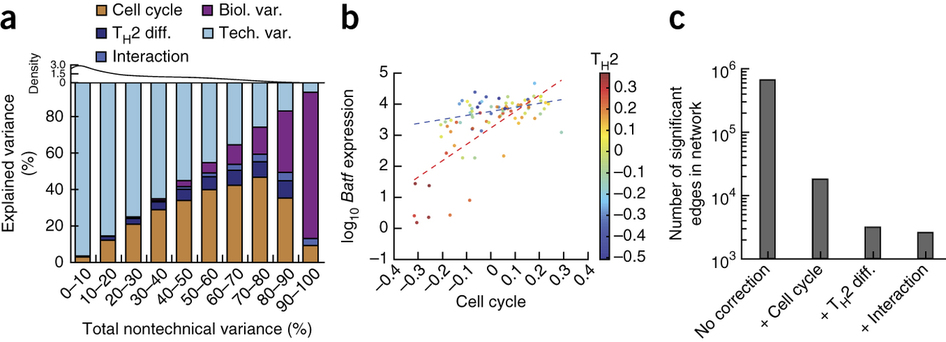
\includegraphics[width=0.8\linewidth]{images/variation.jpg}
%\caption{a) Proportion of variance explained by individual components\\
%b)Interaction between factors for cell cycle and $T_H$2 differentiation: High $T_H$2 implies high Batf expression correlated with higher cell cycle
%c) Number of }
%\end{figure}
%\end{frame}

\begin{frame}
\frametitle{Validation}
\begin{itemize}[<+- | alert@+>]
%\item RNA-seq data from an experiment designed to study the differentiation of T cells into $T_H$2 helper cells
\item Generate single-cel RNA-seq data from mouse embryonic stem cells(mESCs)
\item The status of cell-cycle of each such cell is known apriori(Hoesch staining method)
\item Perform scLVM fitting of the final expression values using an annotated gene set (from GO/Cellbase) known to be associated
with cell cycle
\item The final results are independent of the source of annotation(either GO or CellBase)
\item The results were consistent even if the size of annotated genes was reduced to 10
\item The gold standard and scLVM results are in sync
\end{itemize}
\end{frame}

\begin{frame}
\frametitle{Efficacy: How about just throwing out those known genes?}
If the genes are known to be associated with cell cycle, why not simple throw them out to rule out the 
effect of cell cycle?

A non-linear PCA of datasets with cell-cyclee associated genes thrown out gave a clear separation, and this separation
was later validated to be two different cell cycles $=>$ \textit{scLVM} accounts for the latent factors which
cannot be simply accounted by throwing away those \textit{informative} genes.

\end{frame}

\begin{frame}
\frametitle{Identifying cell populations in differentiating $T_H$2 cells}
Application: RNA-seq experiment to study differentiation of naive T cells into helper cells
\begin{itemize}[<+- | alert@+>]
\item scLVM corrected gene expression levels have significantly low between cell correlations: Majority of the varianceis attributable to cell cycle
\item Significantly corrleated genes post scLVM application were found to be involved in glycolysis and cellular response to IL-4 stimulus(triggers differentiation)
\item To further validate: non linear PCA with and without scLVM correction. Without correction: no obvious subgroups
\item One of the two sub-populations post scLVM correction were found to have genes that marked completion of differentiation

\end{itemize}
\end{frame}

\begin{frame}
\frametitle{Results in a gist}
\begin{itemize}[<+- | alert@+>]
\item Before applying \textit{scLVM} the cells looked like a variable population
\item scLVM corrected expression data showed there existed two sub-populations
\item These two sub-populations were infact found to be associated with T-cell differentiation stages
\item The method is not about single cell transcriptomics. It is a general approach to isolate, model and understand sources of variability
\end{itemize}
\end{frame}

\begin{frame}
\frametitle{Possibilites and limitations}
\begin{itemize}[<+- | alert@+>]
\item It is possible to account for more than one factor, as long as the corresponding annotated gene sets are available
\item When multiple confounding factors are considered, in order to ensure robust analysis it is important to ensure
the statistical significance if the factors are weak or nonindependent
\item No formal tests exist for testing the presence of a particular factor

\end{itemize}
\end{frame}


\begin{frame}%[allowframebreaks]
\frametitle{The underlying model}
Let $N$ = Number of cells \\
$G$ = Number of variable genes(determined using a T-test on pre-processed count data)
$G_h$ = Set of marker genes(cell-cycle related) \\
$Y_h$ = $[y_1, y_2, ... y_h]$ = Vector of gene expressions  where $y_g$ represents gene g's expression acorss cells

\begin{equation}
Y_h = \mu + CU + XW + \psi
\end{equation}
$U,W$ = Weight of linear covariance model where $C$ models $Q$ known covariates and $W$ models unknown covariates.

$\psi$ models the rest of noise

$C,X$ are determined using a bayesian approach assuming both U,W as gaussians prior.

\end{frame}

\begin{frame}%[allowframebreaks]

\begin{equation}
P(Y_h|\sigma_u^2, \nu^2, X, C) = \Pi_{g=1}^{G} N(y_g|\mu_g, {\sigma_u^2CC^T+XX^T+\nu^2} )
\end{equation}
%\end{frame}

%\begin{frame}%[allowframebreaks]
The parameters are then estimated using maximum likelihood approach. Once $XX^T$ is modeled, the genes are modeled
as sume of mean and random effect:

\begin{equation}
y_g = \mu + \sum_{h=1}^Hu_h + \psi_e + \psi_t
\end{equation}

where $P(u_h)=N(\mu_h|0, \sigma_{gh}^2\sigma_h)$, the last two terms accouting for residual and technical noise

and hence:

$y_{corrected} = y_g - y_g^{(hidden)}$
where $y_g^{(hidden)}$ is the posterior estimation:
$y_g^{hidden} = \sigma[\sigma +\nu_g]^{-1}(y_g-\mu_g)$
\end{frame}

\section{Conclusion}
\begin{frame}[fragile]
\frametitle{Conclusion}
\begin{itemize}
\item Heterogeneity in gene expression in single cells can be compromised by factors such as cell-cycle which are often ignored
\item scLVM provides a bayesian approach towards filtering out the effect of confounding variables
\item Counter-intuitively it is easier to cope with \textit{lots} of data that is homogeneous than with limited data that is heterogeneous
\item Apriori knowledge of confounding factor association can help decompose the variance, possibly raveling underlying undiscovered biology
\end{itemize}
\end{frame}
\end{document}
